
\tikzset{eln/.style={midway, font = \Large,inner sep=2pt, outer sep=.30cm}}
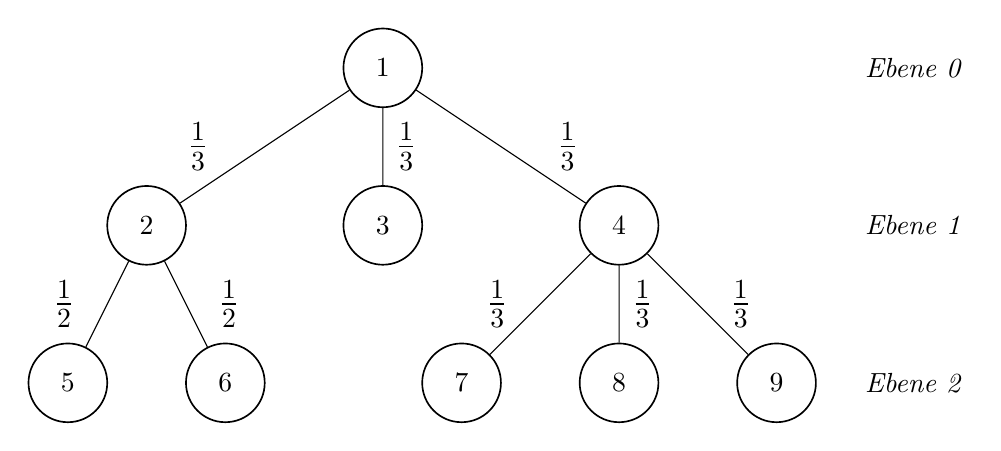
\begin{tikzpicture}[level distance=2cm,
  level 1/.style={sibling distance=3cm},
  level 2/.style={sibling distance=2cm},
  element/.style={circle, draw=black, fill=white, semithick, minimum size=10mm, align=center},
  attribute/.style={ draw=red, fill=white, semithick, minimum size=7mm, align=center},
  textnode/.style={ draw=black, fill=white, semithick, minimum size=7mm, align=center}]
  \node [element](Root){1}
    child {node [element]{2} 
      child {node [element]{5} edge from parent node[left,font = \Large, outer sep=.30cm]{ \( \frac{1}{2} \)} }
      child {node [element]{6} edge from parent node[right,font = \Large, outer sep=.30cm]{ \( \frac{1}{2} \)} }
      edge from parent node[left,font = \Large, outer sep=.60cm]{ \( \frac{1}{3} \)}
    }
    child {node [element]{3} edge from parent node[right,font = \Large, outer sep=0.5mm]{ \( \frac{1}{3} \)}}
    child {node [element]{4}
      child {node [element]{7} edge from parent node[left,font = \Large, outer sep=.30cm]{ \( \frac{1}{3} \)}}
      child {node [element]{8} edge from parent node[right,font = \Large, outer sep=0.5mm]{ \( \frac{1}{3} \)}}
      child {node [element]{9} edge from parent node[right,font = \Large, outer sep=.30cm]{ \( \frac{1}{3} \)}}
      edge from parent node[right,font = \Large, outer sep=.60cm]{ \( \frac{1}{3} \)}
    };
    \begin{scope}[every node/.style={right}]
     \path (Root    -| Root-3-3) ++(5mm,0) node{}  ++(5mm,0) node {\emph{Ebene 0}};
     \path (Root-1  -| Root-3-3) ++(5mm,0) node{}  ++(5mm,0) node{ \emph{Ebene 1}};
     \path (Root-1-1-| Root-3-3) ++(5mm,0) node{}  ++(5mm,0) node {\emph{Ebene 2}};
   \end{scope}
\end{tikzpicture}